% Created 2021-02-26 Fri 10:13
% Intended LaTeX compiler: pdflatex
\documentclass[presentation,dvipdfmx,CJKbookmarks]{beamer}
\usepackage{bxdpx-beamer}
\usepackage{CJKutf8}
\usepackage{atbegshi}
\AtBeginShipoutFirst{\special{pdf:tounicode UTF8-UTF16}} % for UTF-8
\usepackage[utf8]{inputenc}
\usepackage[T1]{fontenc}
\usepackage{graphicx}
\usepackage[export]{adjustbox}
\usepackage{lmodern}
\usepackage{grffile}
\usepackage{longtable}
\usepackage{wrapfig}
\usepackage{rotating}
\usepackage[normalem]{ulem}
\usepackage{amsmath}
\usepackage{textcomp}
\usepackage{amssymb}
\usepackage{capt-of}
\usepackage{hyperref}
 \usepackage{minted}
\usetheme{EastLansing}
\usecolortheme{default}

\date{2021-02-25}


\hypersetup{
 pdfauthor={包昊军},
 pdftitle={seL4\thinspace 介绍},
 pdfkeywords={},
 pdfsubject={},
 pdfcreator={Emacs 27.1 (Org mode 9.3)},
 pdflang={English}}
\begin{document}
\begin{CJK*}{UTF8}{simsun}

\title{seL4\thinspace 介绍}
\subtitle{一个形式化验证的安全微内核}
\author{包昊军}

\maketitle
\begin{frame}{Outline}
\tableofcontents
\end{frame}

\CJKtilde

\section{seL4:安全高性能硬实时的微内核操作系统}
\label{sec:orgcdb9bf7}
\begin{frame}[label={sec:org50f4d5c}]{微内核}
\begin{center}
\includegraphics[width=.9\linewidth]{./images/micro-kernel-structure.ps}
\end{center}
\end{frame}

\begin{frame}[label={sec:org5c881e1}]{微内核与安全性}
\begin{figure}[htbp]
\centering
\includegraphics[width=.6\linewidth]{./Genode_intro.ps}
\caption{Genode\thinspace 操作系统}
\end{figure}
\end{frame}

\begin{frame}[label={sec:org9c6b16f}]{基于\thinspace capbilities\thinspace 的安全性}
\begin{block}{Posix\thinspace 模型}
\begin{itemize}
\item syscall open file X

操作系统提供权限检查
\item client -> server open file X

client\thinspace 对\thinspace X\thinspace 是否有操作权限,操作系统无法强制
\end{itemize}
\end{block}
\end{frame}

\begin{frame}[label={sec:org55161a9}]{Caps\thinspace 模型}
\begin{center}
\includegraphics[width=.9\linewidth]{./images/caps-key.ps}
\end{center}

针对所有资源的操作,均需提供\thinspace caps\thinspace 证明拥有权限
\begin{itemize}
\item 进程间通信
\item 地址空间
\item 中断处理
\item 调度上下文
\end{itemize}
\end{frame}

\begin{frame}[label={sec:org5b7125a}]{高性能}
\begin{itemize}
\item 微内核性能差是一种偏见(Mach)
\item L4\thinspace 系统微内核对\thinspace IPC\thinspace 调用优化(Jochen Liedtke)
\begin{itemize}
\item 优化\thinspace IPC\thinspace 调用开销
\item 微内核减小内存使用,带来\thinspace cache hitrate\thinspace 提升
\end{itemize}
\end{itemize}
\end{frame}

\begin{frame}[label={sec:orgcfb830c}]{硬实时}
\begin{block}{seL4\thinspace 调度策略简单可靠,易分析证明}
\end{block}
\begin{block}{必须考虑中断时延}
\begin{itemize}
\item 一般都是抢占式,即内核态不关中断,只在关键区域短暂关中断
\item seL4\thinspace 是非抢占式的,内核态会关中断
\item 怎么解决中断时延变长的问题?
\end{itemize}
\end{block}
\end{frame}

\begin{frame}[label={sec:org0ff30c1}]{Mixed Criticality System}
\begin{itemize}
\item 不同严重等级的多个系统整合在一起
\item 节省空间、重量、能源
\item seL4\thinspace 实现原理:时间(调度算法)也引入\thinspace Capbility\thinspace 管理
\begin{itemize}
\item \text{\includegraphics[width=1em,valign=t,raise=0.1em,natwidth=48bp,natheight=48bp]{/home/bhj/src/github/Wrench/release/emojis/iphone-new/CROSS_MARK.png}} 时间片 + 优先级(传统方法,会造成资源严重浪费)
\item \text{\includegraphics[width=1em,valign=t,raise=0.1em,natwidth=48bp,natheight=48bp]{/home/bhj/src/github/Wrench/release/emojis/iphone-new/WHITE_HEAVY_CHECK_MARK.png}} 时间片预算 + 优先级 + 预算周期
\pause
\begin{itemize}
\item 预算 = WCET
\item 周期 = Deadline\thinspace 周期
\item 实时性:(预算\thinspace A/周期\thinspace A)+(预算\thinspace B/周期\thinspace B)+\ldots{} < 100\%
\item MCS:A\thinspace 的预算超了,无法完成,A\thinspace 系统故障,不影响其他
\end{itemize}
\end{itemize}
\end{itemize}
\end{frame}


\section{seL4\thinspace 项目}
\label{sec:org6ed3ae4}
\begin{frame}[label={sec:org7ffb8e3}]{seL4\thinspace 官方项目}
\begin{block}{\href{https://docs.sel4.systems/projects/buildsystem/host-dependencies.html}{编译环境准备}}
\end{block}
\begin{block}{sel4-tutorials(入门教程)}
\begin{description}
\item[{github}] \url{https://github.com/seL4/sel4-tutorials}
\item[{文档}] \url{https://docs.sel4.systems/Tutorials/}
\end{description}
\end{block}
\begin{block}{sel4test(unit tests and more)}
\begin{description}
\item[{github}] \url{https://github.com/seL4/sel4test}
\end{description}
\end{block}

\begin{block}{sel4-camkes(微内核嵌入式系统的组件化架构)}
\begin{description}
\item[{文档}] \url{https://docs.sel4.systems/projects/camkes/manual.html}
\end{description}
\end{block}
\end{frame}

\begin{frame}[label={sec:org6d9a9a3}]{seL4\thinspace 社区项目}
\begin{block}{genode on sel4}
\begin{itemize}
\item 一个开源的「操作系统框架」
\item sel4\thinspace 移植的过程写了\thinspace 3\thinspace 篇文章
\begin{enumerate}
\item \href{https://genode.org/documentation/articles/sel4\_part\_1}{两个交替执行计算和打印的线程}
\item \href{https://genode.org/documentation/articles/sel4\_part\_2}{IPC\thinspace 和虚拟内存实验}
\item \href{https://genode.org/documentation/articles/sel4\_part\_3}{移植核心组件}
\end{enumerate}
\end{itemize}
\end{block}
\begin{block}{\href{https://github.com/PolySync/cargo-fel4}{fel4}}
\begin{itemize}
\item 直接在\thinspace sel4\thinspace 上运行嵌入式\thinspace rust\thinspace 程序
\item 项目已过时,需要修改源码之后才能运行
\end{itemize}
\end{block}
\begin{block}{\href{https://gitlab.com/arm-research/security/icecap/icecap/}{icecap}}
\begin{itemize}
\item Arm Research\thinspace 的\thinspace sel4 rust\thinspace 项目
\end{itemize}
\end{block}
\end{frame}

\begin{frame}[label={sec:org2302d25}]{项目中使用组件框架的建议}
\begin{block}{seL4 API\thinspace 易用性差(重点在于形式化验证)}
\end{block}
\begin{block}{所以需要使用组件框架,重点关注业务逻辑}
\end{block}
\begin{block}{\href{https://sel4.systems/About/seL4-whitepaper.pdf}{两个主要的组件框架:camkes\thinspace 和\thinspace genode}}
\begin{itemize}
\item camkes\thinspace 主要用于静态系统:组件预定义,启动之后不再变化
\item genode\thinspace 更强大通用,但无法使用\thinspace sel4\thinspace 全部安全特性
\item 挑战:如何同时使用\thinspace genode\thinspace 和\thinspace camkes
\end{itemize}
\end{block}
\begin{block}{\href{https://docs.sel4.systems/projects/sel4/frequently-asked-questions.html}{libsel4utils}}
\begin{itemize}
\item 提供了一些有用的抽象,比如进程,但更偏底层
\end{itemize}
\end{block}
\end{frame}

\section{sel4\thinspace 研究方向}
\label{sec:orgbe62c75}
\begin{frame}[label={sec:org41d1d19}]{\href{https://ts.data61.csiro.au/students/theses.pml.html}{研究项目}}
\begin{itemize}
\item 多核、IPC\thinspace 性能优化
\item Secure, Android-based OS for IoT
\item \href{https://ts.data61.csiro.au/projects/TS/realtime.pml.html}{seL4 AUTOSAR}
\item Shared resources in an microkernel-based OS(用\thinspace camkes\thinspace 实现文件系统、网络协议栈)
\item Linux as a component(camkes-vm)
\end{itemize}
\end{frame}
\begin{frame}[label={sec:org61e8bec}]{\href{https://github.com/seL4/docs/blob/master/SuggestedProjects.md}{Github\thinspace 项目建议}}
\begin{itemize}
\item 移植\thinspace minix3\thinspace 到\thinspace sel4
\item 移植\thinspace Doom\thinspace 到\thinspace sel4
\end{itemize}
\end{frame}

\section{sel4\thinspace 动态}
\label{sec:org4e0d6df}
\begin{frame}[label={sec:orge4a78ce}]{sel4\thinspace 动态}
\begin{itemize}
\item 2020\thinspace 年\thinspace 4\thinspace 月,成立\thinspace seL4\thinspace 基金会,由\thinspace Linux\thinspace 基金会托管(\href{https://microkerneldude.wordpress.com/2020/04/07/the-sel4-foundation-what-and-why/}{sel4\thinspace 原作者博客})
\item 2021\thinspace 年\thinspace 2\thinspace 月,FOSDEM 2021
\end{itemize}
\end{frame}
\begin{frame}[label={sec:org32b56c5}]{sel4 RFC(FOSDEM 2021)}
\begin{center}
\includegraphics[width=.9\linewidth]{./images/rfc-for-core.ps}
\end{center}
\begin{itemize}
\item Core、Core Platform
\begin{itemize}
\item Core\thinspace 整个\thinspace seL4\thinspace 核心系统
\item Core Platform\thinspace 操作系统特性和开发平台
(比如\thinspace Posix\thinspace 就是一种操作系统特性)
\end{itemize}
\end{itemize}
\end{frame}

\begin{frame}[label={sec:org07c2f00}]{sel4 multi-server OS}
\begin{center}
\includegraphics[width=.9\linewidth]{./images/multi-server.os.ps}
\end{center}
\end{frame}

\begin{frame}[label={sec:orgd2be28c}]{sel4 multi-server OS}
\begin{center}
\includegraphics[width=.9\linewidth]{./images/multi-server.os.2.ps}
\end{center}
\end{frame}

\section{Qemu gdb\thinspace 调试\thinspace Demo}
\label{sec:org248c233}
\begin{frame}[label={sec:orgcf654ce},fragile]{使用\thinspace Qemu、gdb\thinspace 调试\thinspace sel4\thinspace 内核与应用}
 \begin{block}{Gdb\thinspace 调试方式启动\thinspace Qemu\thinspace 仿真}
\begin{minted}[]{sh}
./simulate  --gdb
\end{minted}
\end{block}

\begin{block}{Gdb\thinspace 调试\thinspace kernel}
\begin{minted}[]{sh}
./launch_gdb -f kernel/kernel.elf
(gdb) b seL4_MessageInfo_new
\end{minted}
\end{block}

\begin{block}{Gdb\thinspace 调试\thinspace sel4\thinspace 应用}
\begin{minted}[]{sh}
./launch_gdb -f dynamic-4
(gdb) b main
\end{minted}
\end{block}
\end{frame}

\section{参考链接}
\label{sec:orga059d9d}
\begin{frame}[label={sec:org3b276f7}]{参考链接}
\begin{itemize}
\item \href{https://docs.sel4.systems/projects/sel4/api-doc.html}{官网}
\item \href{https://sel4.systems/About/seL4-whitepaper.pdf}{白皮书}
\item \href{https://microkerneldude.wordpress.com/2020/04/07/the-sel4-foundation-what-and-why/}{sel4\thinspace 原作者博客}
\end{itemize}
\end{frame}

\begin{frame}[label={sec:org359e13e}]{谢谢聆听}
元宵节快乐&周末愉快!
\end{frame}
\end{CJK*}
\end{document}
